\documentclass[conference]{IEEEtran}
\usepackage{graphicx}
\usepackage{booktabs}
\usepackage{amsmath}
\usepackage{array}
\usepackage{url}
\usepackage[hidelinks,pdfauthor={Anonymous},pdftitle={Leakage-Safe Three-Way Decision Policy Selection for Cross-Platform Profile Identity Resolution},pdfsubject={Anonymous conference submission}]{hyperref}

\title{Leakage-Safe Three-Way Decision Policy Selection for Cross-Platform Profile Identity Resolution}
\author{\IEEEauthorblockN{Anonymous Submission}}

\begin{document}
\maketitle

\begin{abstract}
Social platforms hold fragmented and incomplete views of the same person. Cross-platform identity resolution first retrieves plausible profile pairs, then estimates whether each pair belongs to one entity. A probability alone, however, does not determine whether a system should merge, defer, or reject a pair. We study a leakage-safe pipeline that maps calibrated pair probabilities to MATCH, REVIEW, and NO\_MATCH decisions. A controlled ablation separates fixed thresholds (B0), validation tuning of the same threshold family (B1), expansion to a four-parameter policy searched by Sobol points (B2), and the identical expanded policy searched by a genetic algorithm (B3). Three entity-disjoint outer partitions use physically sealed test labels and equal 12,000-evaluation B2/B3 budgets. Validation tuning improves mean workflow F1 from 0.8510 to 0.8910 and lowers illustrative utility loss from 2364.2 to 1864.6. Policy expansion changes the operating trade-off only slightly. Sobol and genetic search are nearly indistinguishable (F1 0.8901 versus 0.8903; loss 1860.0 versus 1858.2), so the evidence does not support a GA-specific advantage. Candidate retrieval covers 25,931 of 29,243 cross-platform positives (88.6742\%), imposing an end-to-end recall ceiling.
\end{abstract}

\section{Introduction}
A person may maintain profiles on several online platforms, using different usernames, names, biographies, and locations. Identity resolution attempts to determine which records refer to the same underlying entity. For social profiles, this problem combines sparse fields, platform-specific conventions, and a comparison space that grows quadratically. Prior work treats user identity linkage as a distinct cross-network problem and uses profile, behavioral, or network evidence \cite{shu2017uilreview,linkSocial2018,yao2023profile}.

A practical pipeline cannot compare every cross-platform pair. It first retrieves a candidate set, represents each candidate pair, and estimates a match probability. Yet a probability is not an operational action. Incorrect automatic merges and missed links have different consequences, while uncertain cases may be deferred. This motivates a three-way output: MATCH, REVIEW, or NO\_MATCH. Such reject and review regions have roots in probabilistic linkage and reject-option decision theory \cite{fellegi1969theory,chow1970reject,ouyang2019threeway}.

This paper asks three bounded questions. First, does adding one frozen semantic cosine feature improve a handcrafted pair model? Second, what is gained by validation-tuning a three-way decision policy and then expanding its policy class? Third, when policy class, data, objective, and evaluation budget are held fixed, does a genetic algorithm (GA) improve over deterministic Sobol search? We answer with three repeated entity-disjoint partitions, role-specific development labels, physically sealed test labels, and explicit accounting for positives missed by candidate generation.

The contribution is empirical rather than a claim of a new classifier, embedding, or optimizer: (i) a leakage-safe evaluation architecture for staged identity resolution; (ii) a controlled B0--B3 comparison that separates tuning, policy-class expansion, and optimizer choice; and (iii) workflow metrics that include the candidate-retrieval ceiling. The results support validation-selected three-way decisions, but not a GA-specific headline claim.

\section{Related Work}
\textbf{Identity linkage and entity resolution.} Fellegi and Sunter formalized probabilistic record linkage with match, possible-match, and non-match regions \cite{fellegi1969theory}. Cross-platform user linkage extends the problem to heterogeneous social profiles \cite{shu2017uilreview,linkSocial2018}. Profile-field approaches remain relevant when graph or behavioral data are unavailable \cite{yao2023profile}.

\textbf{Candidate generation.} Blocking reduces the otherwise quadratic comparison space, but retrieval errors cannot be repaired by downstream classification \cite{papadakis2021blocking,li2020blocking}. Learned blocking offers an alternative design space \cite{thirumuruganathan2021deepblocker}; our experiment instead freezes a deterministic candidate generator and exposes its misses in workflow recall.

\textbf{Pair representation and calibration.} Neural entity matching and pretrained language models can capture semantic evidence beyond string similarities \cite{barlaug2021survey,li2020ditto}. We test a narrower intervention: one frozen MiniLM cosine feature appended to 17 handcrafted attributes. Since policy thresholds act on probabilities, we use isotonic calibration fitted on a separate role; calibration of supervised classifiers is a well-established concern \cite{niculescu2005calibration}.

\textbf{Review decisions and optimization.} Three-way record linkage and reject-option learning explicitly represent uncertainty \cite{ouyang2019threeway,hendrickx2024reject}. Human-in-the-loop ER systems additionally study interaction and explanation \cite{qian2019systemer}; our REVIEW output is only an offline decision and is not evidence about human performance. GA-based ER has precedent \cite{sun2017gaer}. Consequently, our optimizer claim is deliberately narrow and requires a same-class, same-budget comparison.

\section{Cross-Platform Identity Resolution Pipeline}
Figure~\ref{fig:pipeline} gives the complete system. Profiles from Twitter, Google+, and Instagram enter candidate generation. Each candidate receives 17 deterministic handcrafted features: username and full-name string similarities, an unconditional maximum cross-field name similarity, biography overlap and availability, location similarities, platform agreement, and length/prefix indicators. The 18-feature representation adds one cosine between normalized embeddings of full name, biography, and location. The embedding model is fixed and receives no task labels.

A gradient-boosting classifier produces a pair score, and isotonic regression maps it to a calibrated probability. The downstream policy then emits MATCH, REVIEW, or NO\_MATCH. Exact-tier candidate pairs bypass classifier scoring and enter the workflow as MATCH. Blocking-missed known positives enter only final workflow evaluation as NO\_MATCH; they are never synthesized as classifier inputs.

\begin{figure*}[t]
\centering
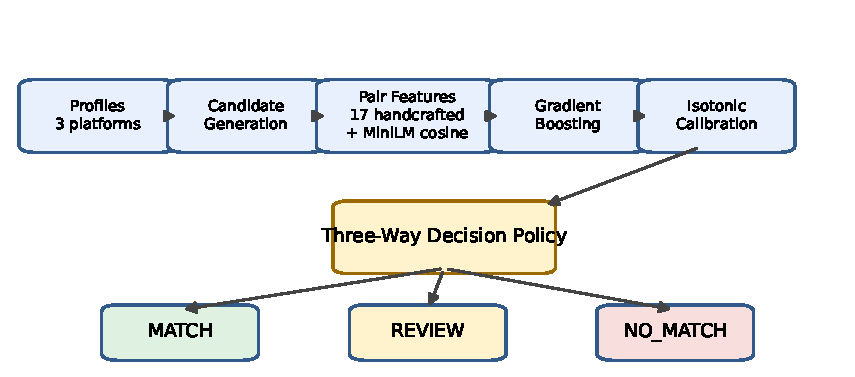
\includegraphics[width=0.94\textwidth]{figures/system_pipeline.pdf}
\caption{Staged cross-platform identity-resolution pipeline. MiniLM contributes one semantic feature inside pair representation; it is not a separate decision system.}
\label{fig:pipeline}
\end{figure*}

\section{Methodology}
\subsection{Dataset and Candidate Generation}
We use a local normalized derivative of the public LinkSocial corpus \cite{linkSocial2018}. It contains 36,804 eligible profiles after the frozen validity filters. Ground truth is defined by shared source entity folders, but raw names, usernames, biographies, URLs, image references, entity identifiers, and pair identifiers are excluded from publication artifacts.

The eligible cross-platform universe contains 449,149,239 possible pairs and 29,243 labeled positives. Candidate generation returns 12,403 exact-tier and 2,073,842 model-scored pairs, for 2,086,245 workflow candidates. It covers 25,931 positives and misses 3,312, giving retrieval recall $25{,}931/29{,}243=88.6742\%$ and candidate-space reduction 99.5355\%. Four same-platform positives are excluded from the cross-platform denominator.

\subsection{Pair Representation}
GB-17 uses the 17 handcrafted features described above. The corrected \texttt{name\_sim} is always the maximum Jaro--Winkler similarity across username/full-name cross-combinations when values exist; it has no predecessor-score gate. GB-18 is exactly GB-17 plus one normalized MiniLM cosine. Both representations use identical candidate keys and split roles.

\subsection{Classification and Calibration}
For each outer partition and feature set, we fit \texttt{GradientBoostingClassifier} with 300 trees, learning rate 0.05, maximum depth 6, and random state 42. TRAIN retains all positives and a deterministic 3:1 negative sample. A distinct isotonic regressor with out-of-bounds clipping is fitted on CALIBRATION only. GB-17 and GB-18 are trained and calibrated independently.

\subsection{Three-Way Decision Policies}
For decisions $d\in\{\mathrm{MATCH},\mathrm{REVIEW},\mathrm{NO\_MATCH}\}$, policy selection minimizes
\begin{equation}
U=2\,FP+FN+0.1\,REVIEW.
\end{equation}
The coefficients define an illustrative engineering trade-off, not measured financial cost. The controlled methods are summarized in Table~\ref{tab:baselines}. B0 uses fixed thresholds $(0.98,0.95)$. B1 tunes the same two-threshold family. B2 and B3 share parameters $[t_m,t_r,c_p,c_d]$: outside the probability band they match or reject; inside it, high name similarity promotes and low name similarity demotes, otherwise REVIEW is retained. Bounds are frozen before evaluation.

\begin{table}[t]
\caption{Controlled decision-policy comparison.}
\label{tab:baselines}
\centering
\begin{tabular}{llllr}
\toprule
ID & Policy & Tune? & Search & Eval.\\
\midrule
B0 & Fixed simple & No & None & 0\\
B1 & Simple & Yes & Determ. & 12,000\\
B2 & Expanded 4-par. & Yes & Sobol & 12,000\\
B3 & Same expanded & Yes & GA & 12,000\\
\bottomrule
\end{tabular}
\end{table}

\section{Leakage-Safe Experimental Design}
\subsection{Entity-Disjoint Roles}
Each seed (101, 202, 303) deterministically assigns complete entities, not pair rows, to TRAIN, CALIBRATION, POLICY\_VALIDATION, or SEALED\_TEST. Cross-role pairs are discarded. Thus profiles from one person cannot occur in more than one role. Development artifacts contain labels only for the first three roles, and each consumer requests its own role explicitly.

SEALED\_TEST labels reside in physically separate files. Models and calibrators are fitted, B1--B3 are selected, and label-free sealed predictions are hashed before FINAL\_EVALUATION opens those files through a lazy adapter. Figure~\ref{fig:leakage} illustrates the boundary. Instrumentation recorded zero pre-final test-label reads in all three runs.

\begin{figure*}[t]
\centering
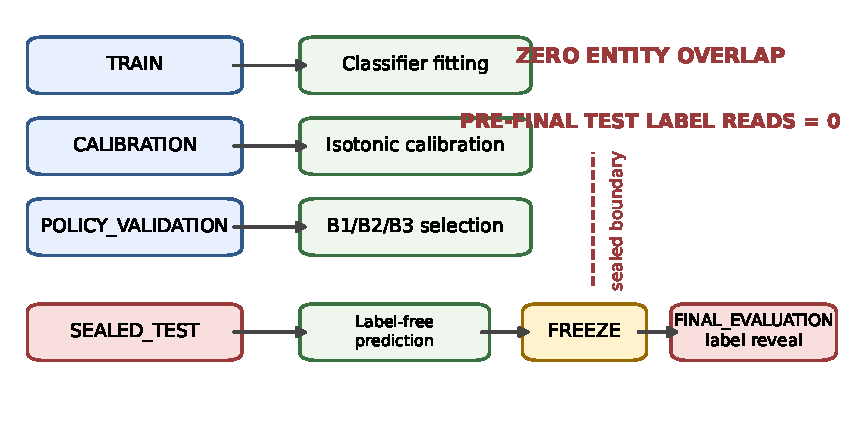
\includegraphics[width=0.92\textwidth]{figures/leakage_safe_design.pdf}
\caption{Entity-disjoint roles and physical test-label boundary. Test predictions are frozen before the final keyed label reveal.}
\label{fig:leakage}
\end{figure*}

\subsection{Controlled B0--B3 Ablation}
B0 to B1 changes only validation tuning within the simple family. B1 to B2 changes the policy class under deterministic search. B2 to B3 changes only optimizer choice: both use the same validation rows, bounds, four-parameter decision function, objective, and exactly 12,000 realized evaluations. Ties retain the first candidate in deterministic generation order.

\subsection{Metrics}
We report precision, recall, F1, FP, FN, REVIEW, and $U$. All are workflow metrics unless explicitly marked model-scored. Workflow rows combine exact-tier decisions, scored candidates, and blocking misses. Metrics were independently recomputed from frozen row-level Parquet artifacts and matched runner summaries exactly. Across three outer partitions we report means and sample standard deviations.

\section{Results and Discussion}
\subsection{Semantic Feature Effect}
Table~\ref{tab:aggregate} reports workflow results. Adding the semantic cosine under the same B0 policy changes mean F1 from $0.8494\pm0.0257$ to $0.8510\pm0.0235$. Mean recall rises by 0.0020 and mean $U$ worsens by 12.2. These differences are small relative to between-partition variation. The experiment therefore does not establish a substantive benefit from the single MiniLM feature; richer semantic modeling remains untested.

\begin{table*}[t]
\caption{Workflow metrics over seeds 101, 202, and 303 (mean $\pm$ sample SD). Lower $U$ is better.}
\label{tab:aggregate}
\centering
\begin{tabular}{lrrrrrrr}
\toprule
Method & Precision & Recall & F1 & FP & FN & Review & $U$\\
\midrule
GB-17+B0 & .9863$\pm$.0024 & .7466$\pm$.0405 & .8494$\pm$.0257 & 89.0$\pm$25.1 & 2137.3$\pm$211.9 & 366.3$\pm$461.0 & 2352.0$\pm$212.3\\
GB-18+B0 & .9870$\pm$.0080 & .7486$\pm$.0387 & .8510$\pm$.0235 & 88.0$\pm$56.5 & 2171.3$\pm$251.8 & 168.7$\pm$288.7 & 2364.2$\pm$212.0\\
GB-18+B1 & .9834$\pm$.0047 & .8146$\pm$.0008 & .8910$\pm$.0024 & 115.3$\pm$30.1 & 1557.7$\pm$31.1 & 762.3$\pm$178.1 & 1864.6$\pm$45.9\\
GB-18+B2 & .9844$\pm$.0029 & .8124$\pm$.0041 & .8901$\pm$.0016 & 107.7$\pm$21.7 & 1560.3$\pm$32.6 & 843.7$\pm$260.7 & 1860.0$\pm$27.1\\
GB-18+B3 & .9844$\pm$.0029 & .8127$\pm$.0037 & .8903$\pm$.0015 & 107.7$\pm$21.7 & 1557.7$\pm$31.1 & 852.3$\pm$263.9 & 1858.2$\pm$30.0\\
\bottomrule
\end{tabular}
\end{table*}

\subsection{Validation Tuning}
B0 to B1 isolates validation tuning. Mean recall increases from 0.7486 to 0.8146, F1 from 0.8510 to 0.8910, and $U$ decreases by 499.6. The gain is consistent with moving uncertain positives away from NO\_MATCH: mean FN falls by 613.7. The trade-off is 27.3 more FP and 593.7 more REVIEW cases on average. Thus tuning improves the declared objective and F1, but increases both false-positive and review burdens.

\subsection{Expanded Policy Effect}
B1 to B2 introduces name-based promotion/demotion while retaining deterministic Sobol selection. Mean $U$ improves only 4.5, while F1 declines 0.0009 and recall declines 0.0022. FP falls by 7.7, FN rises by 2.7, and REVIEW rises by 81.3. The expanded class therefore yields a small objective-specific trade-off, not a general accuracy improvement.

\subsection{Sobol versus GA}
B2 and B3 are nearly indistinguishable. Mean F1 differs by 0.00014 and mean $U$ by 1.8. GA improves $U$ by 5.5 in seed 101, ties exactly in seed 202, and is 0.1 worse in seed 303. Since improvement is neither clear nor consistent, CLAIM\_PROTOCOL requires that we reject a GA-specific benefit claim. The defensible conclusion is that policy selection matters; the chosen optimizer does not materially change the observed result in this low-dimensional search.

\subsection{Candidate Retrieval Ceiling}
The final policy cannot recover pairs absent from the candidate set. Across the global cross-platform universe, 3,312 of 29,243 positives are blocking misses, so candidate recall is 88.6742\%. In the three sealed roles, blocking misses number 1,034, 1,014, and 1,007. These rows are counted as workflow FN for every method, explaining why model-scored performance alone would overstate end-to-end recall.

\begin{table}[t]
\caption{Per-partition F1 / $U$ for the controlled policies.}
\centering
\begin{tabular}{lrrr}
\toprule
 & Seed 101 & Seed 202 & Seed 303\\
\midrule
B0 & .8253 / 2568.2 & .8560 / 2379.4 & .8716 / 2145.0\\
B1 & .8915 / 1856.9 & .8884 / 1913.8 & .8932 / 1823.0\\
B2 & .8891 / 1832.4 & .8893 / 1861.2 & .8920 / 1886.5\\
B3 & .8896 / 1826.9 & .8893 / 1861.2 & .8920 / 1886.6\\
\bottomrule
\end{tabular}
\end{table}

\section{Limitations and Threats to Validity}
The study uses one historical corpus spanning three now-historical social platforms and only three deterministic outer partitions; it does not establish external generalization. Candidate retrieval fixes an 88.6742\% ceiling and may induce selection effects. Dataset hosting was verified, but a machine-readable reuse license, redistribution permission, collection/Terms-of-Service evidence, consent process, and ethics/IRB documentation were not; consequently, only code, hashes, and aggregates should be released pending clarification.

The utility coefficients are illustrative rather than elicited from users or measured in deployment. REVIEW is an offline label: no human-review workload, accuracy, agreement, or latency was studied. No downstream CRM agent, customer conversion, lead scoring, or business outcome was evaluated. The semantic intervention is only one frozen cosine feature and showed no substantive benefit. The expanded policy offered only a small objective-specific change, and GA did not consistently beat Sobol. Finally, tuning raised false positives and review volume relative to B0, which may be unacceptable under other operating preferences.

\section{Conclusion}
A leakage-safe, staged evaluation shows that validation-selected three-way decision policies can materially improve the declared operating trade-off for cross-platform profile linkage. The major gain comes from tuning a simple policy: mean F1 rises from 0.8510 to 0.8910 and illustrative utility loss falls by about 500. Expanding the policy class has a small effect, while equal-budget Sobol and GA search are effectively similar. A single MiniLM cosine likewise provides no substantive improvement. These negative and positive findings narrow the claim: careful role separation, sealed evaluation, controlled policy selection, and retrieval-aware metrics matter more here than a particular semantic feature or optimizer.

\bibliographystyle{IEEEtran}
\bibliography{references}
\end{document}
